%%%%%%%%%%%%%%%%%%%%%%%%%%%%%%%%%%%%%%%%%%%%%%%%%%%%%%%%%%%%%%%%%%% 
%                                                                 %
%                           INLEIDING                             %
%                                                                 %
%%%%%%%%%%%%%%%%%%%%%%%%%%%%%%%%%%%%%%%%%%%%%%%%%%%%%%%%%%%%%%%%%%% 


\chapter{Ontwerpproces}

In dit hoofdstuk worden de ondernomen stappen besproken bij het ontwerpen van een interface die kristalstructuren, in de vorm van een CIF-bestand, kan visualiseren in Blender. Een meer gedetailleerde beschrijving van dit proces kan worden gevonden in hoofdstuk vier.
In de eerste sectie zal worden uitgelegd hoe, met behulp van een parser, een programma in Python kan geschreven worden dat de gegevens uit een CIF-bestand kan omzetten in verwerkbare data en deze opslaat in geschikte datastructuren.  



\section{Van cif naar py}

\subsection{Zelf een parser ontwerpen}
In de vierde sectie van hoofdstuk twee werd er reeds aangehaald wat er allemaal komt kijken bij het ontwerpen van een parser. Het is gelukt een programma[Bijlage C] te ontwerpen dat alle CIF-bestanden kan inlezen die te vinden zijn op de kristallografische databank van het IZA. Dit is omdat deze allemaal dezelfde textstructuur hebben. Bestanden uit databanken die werken met een andere structuur kunnen gemisinterpreteerd worden waardoor de parser nutteloos is. Het is mogelijk het programma aan te passen zodat, ongeacht de structuur van het CIF-bestand, een juiste interpretatie van de data kan gedaan worden. Dit zou echter veel tijd vergen en zal, in belang van dit onderzoek, niet worden gedaan. In de plaats zal er gewerkt worden met een reeds functionerende CIF-parser.
 

\subsection{Inlezen van CIF}
Het inlezen van een CIF-bestand zal worden gedaan worden met behulp van de PyCIFRW parser, die besproken wordt in het tweede hoofdstuk van deze tekst, en Python3 als programmeertaal. De volledige broncode van het programma[Bijlage D] en een voorbeeld van een CIF-bestand[Bijlage B] kan worden gevonden in de bijlages.

\par
Vooraleer er data kan worden ingelezen dienen er datastructuren gemaakt te worden waarin deze kan worden opgeslagen. Zo een datastructuur noemt men een class en het werken hiermee wordt object georiënteerd programmeren genoemd. Enkele voordelen dat dit biedt over de gewoonlijke, imperatieve, methode van programmeren, zijn overzichtelijkheid, herbruikbaarheid van classes, een extra laag van veiligheid doordat de data niet rechtstreeks kan worden aangepast. Figuur[3.1] wordt een klassendiagram genoemd, en geeft de algemene opbouw het programma aan de hand van de gebruikte datastructuren, methodes, modules en hun onderlinge relaties. Uit dit diagram kan er geïnterpreteerd worden hoe de data uit het CIF-bestand met behulp van de PyCIFRW-parser wordt omgezet in de verschillende datastructuren welke nadien kunnen worden gevisualiseerd in Blender. 

\begin{figure}[]
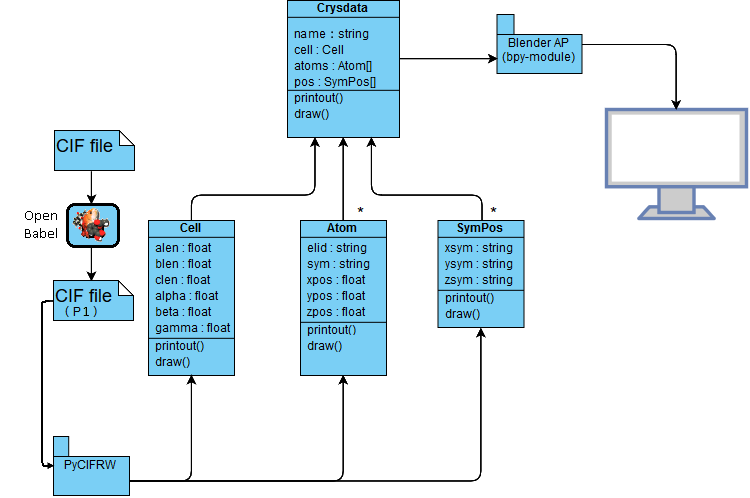
\includegraphics[scale=0.8]{ClassDiagram.png}
\caption{Klassendiagramma van het ontwerp van deze thesis}
\end{figure}

\par  
De broncode van het programma dat een CIF-bestand inleest en in datastructuren omzet kan gevonden worden tussen de bijlagen van deze tekst.[Bijlage D]
